\documentclass[11pt]{article}

\usepackage{amssymb}
\usepackage{setspace}
\usepackage{amsmath}
\usepackage[T1]{fontenc}
\usepackage[utf8]{inputenc}
\usepackage{graphicx}
\usepackage[swedish]{babel}
\usepackage{fixltx2e}
\usepackage{subcaption}
\usepackage{placeins}
\usepackage{fancyhdr}
\usepackage{wrapfig}
\usepackage{tikz}
\usepackage{listings}
\usepackage{hyperref}

\setlength{\intextsep}{5pt}
\setlength{\textfloatsep}{5pt}

\pagestyle{fancy}
\fancyhf{}
\rhead{SI1121}
\chead{\textbf{Kvävelaboration}}
\lhead{Termodynamik}


\begin{document}

\begin{titlepage}
	\centering
	{\scshape\LARGE Kvävets ångbildningsvärme och ”Hemliga lådan” \par}
	{\scshape En introduktion för laborationsassistenter \par}
	\vspace{4cm}
	{\scshape\Large Termodynamik \\ SI1121\par}
	\vspace{2cm}
	\vfill
% Bottom of the page
	{\large \today\par}
\end{titlepage}

% -------- Section --------
\section{Säkerhet}
 
\begin{itemize}
    \item Det är viktigt att bara assistenten hanterar kvävet.
    \item Ta inte i kvävet
    \item Använd skyddsglasögon
    \item Då kvävet är i flytande form så sugs det upp av porösa material såsom kläder, trasor osv.
    \item Viktigt att inte starta nätaggregatet innan resistorn förs ner i kvävet. (Värmeöverföring $\propto \Delta $T, gasen som bildas måste ta vägen någonstans och kommer därför potentiellt få resistorn att åka ur kärlet och skada dig eller närmaste student)
    \item Täck ej över behållaren
    \item Var försiktig så inte kretsen kortsluts mot behållarens väggar
    \item Assistenten är den som startar kretsen
\end{itemize}

\section{Studentens arbetsuppgifter}

\begin{itemize}
    \item Bestämma kvävets ångbildningsentalpi
    \item Uppskatta felkällor
    \item Sätt ihop kretsen enligt figur från labbpeket
    \item När studenten tror att kretsen är ihopsatt så frågar hen efter assistenten för kontroll
    \item Se till att ingen ström är på och för \emph{sakta} ner resistorn i behållaren
    \item Mät massan av kvävet med hjälp av vågen en gång per minut, i fem minuter per effekt för åtta effekter. Effekterna\footnote{Glöm ej $P = U \cdot I$} $P = [0.2, 0.5, 1, 1.5, 2, 5, 10, 20]$\footnote{Dessa värden är valda så att man får en ganska jämn fördelning för $1/P$} W. Starta med dem låga effekterna då kvävet snabbt kokar bort annars
    \item När alla mätvärden är tagna så ska studenterna rita ut på millimeterpapper\footnote{Minustecket är för att $\dot m$ är negativ} $- \frac{P}{\dot m}$ [kJ/kg] mot $\frac{1}{P}$ [s/J]
    \item När alla har fått kväve och börjat mäta kan hemliga lådan starta
\end{itemize}

\section{Hemliga lådan}

En student ur varje grupp får följa med ner till assistentrummet där hemliga lådan utförs. Detta upprepas tills alla har gjort uppgiften. Den går ut på att försöka mäta den mänskliga värmeeffekten ($\approx 1$ W/kg). Till hjälp har de en låda med en fläkt, en 75 W lampa, och en temperatursensor. Fläkten är till för att jämt fördela värmet i lådan.

Det finns många sätt att lösa denna uppgift men här är ett;

Tänd lampan och vänta tiden $t$. Lampan kommer då värma lådan med effekten $P_l$ och öka temperaturen $\Delta \text T_l$. Låt lådans totala mängd luft ha massan $m_{luft}$, och dess specifika värmekapacitet $c_{luft}$.

\begin{equation*}
    P_l = \frac{Q}{t} = \frac{m_{luft} c_{luft} \Delta \text T_l}{t}
\end{equation*}

På samma sätt med en människa i lådan. Vi antar här att skillnaden i massa mellan människan och luften som människan trycker ut ur lådan är liten.

\begin{equation*}
    P_m = \frac{Q}{t} = \frac{m_{luft} c_{luft} \Delta \text T_m}{t}
\end{equation*}

Dessa uttryck kan divideras för att få följande

\begin{equation*}
    P_m = P_l \frac{\Delta \text T_m}{\Delta \text T_l}
\end{equation*}

Detta tar såklart olika lång tid att lista ut, men 15 minuter för att tänka och 10 minuter för att mäta brukar fungera bra.

\section{Resultat och teori}

I Figur 1 visas studenters data tagna från laborationstillfällen under år 2017. Den heldragna plotten motsvarar ungefär den trend som datan borde följa. Vi ser att det riktiga värdet $H = 198.57$ kJ/kg enligt \href{https://en.wikipedia.org/wiki/Nitrogen}{\textbf{wikipedia}}.

\begin{figure}[h]
\center
    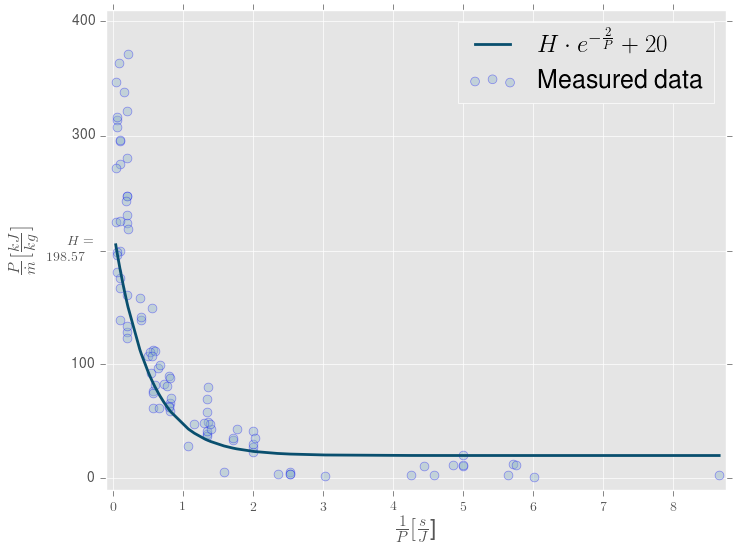
\includegraphics[width = .75\linewidth]{nitrogenEnthalpy.png}
    \caption{Plot $- \frac{P}{\dot m}$ mot $\frac{1}{P}$.}
\end{figure}

Vi ser också att kurvan ej går mot noll då $P \to 0$. Detta är då omgivningens påverkan inte är noll. Däremot så är den konstant. Detta då värmeöverföringen är $\propto$ arean (där värmeöverföringen sker), temperaturskillnaden (mellan omgivning och kväve), samt någon värmeöverföringskonstant $c$. Vi får således

\begin{equation*}
    \text{Totala tillförda värmet} = \langle P \rangle t + \underbrace{ c A \Delta \text T }_{C_0} = \langle P \rangle \left (t + \frac{C_0}{\langle P \rangle} \right ) \stackrel{P \gg 1}{\approx} \langle P \rangle t
\end{equation*}

Alltså påverkar omgivningen relativt mindre då vi ökar $P$. På så sätt kan slutsatsen dras att då $P \to \infty \Rightarrow \frac{1}{P} \to 0$ är där det sanna värdet för ångbildningsentalpin hittas.


\section{FAQ}



\end{document}
